\chapter{Methodology}

It is worth noting that the structure of this chapter is highly general and can be modified to suit specific needs. For example, in a Computer Vision and Deep Learning thesis, you may want to describe the proposed method(s).

\section{Requirements}

\lipsum  % Replace with your text



\section{Particle Swarm Optimization}


\subsection{Introduction to Particle Swarm Optimization}

Particle Swarm Optimization (PSO) is an Optimization approach originally proposed by Kennedy and Eberhart in 1995 \cite{Tesi-3.3}. The idea was to replicate the behaviour of certain animal species which moves in groups, like flocks of birds or shoal of fishes.
\\[0.3cm]The reason is the belief that each singular individual in the group can profit form the experience of all other members; basically, each individual can benefit from what he learns from other individuals, and in the same way, it can share its discoveries to the other individuals \cite{Tesi-3.1}

\subsubsection{Particle Swarm Optimization as an Optimization Problem}

Translating this behaviour into specific terms, each individual can be interpreted as an agent which “flies” in the Search Space, where each physical position is a candidate solution in the n-dimensional Search Space, and the best solution found by the whole group is the best solution.
\\[0.3cm]The best solution found by the whole group will probably not be the real global optimal solution but is a solution which is near the global optimal.

\myparagraph{Formalization of Particle Swarm Optimization:}
The goal of the Particle Swarm Optimization, as all Optimization problem, is to find value which maximizes (or minimizes) the value of an objective (or Fitness) function $f$.
\\[0.3cm]Where $f$ is defined on a Search Space {$\textbf{X}$}, the multi-dimensional vector representing all the possible solutions in the defined limits.
The PSO algorithm will return the vector $X$, which represent a single solution, which maximizes (or minimizes) the value of $f$.

\myparagraph{General Procedure of PSO:}
To find the maximum (or minimum) of the Fitness function $f$, of course the best solution would be to perform an exhaustive search on all the possible solutions. This approach is of course too computationally expensive, and basically unapplicable to higher-dimensional spaces \cite{Tesi-3.1}.
\\[0.3cm]Therefore, in PSO, the same way as a flock of birds searches for food, moving in the air, the algorithm starts with a number of random points in the search spaces, which are called Particles, and have them look for an optimal value by roaming in random directions.
\\[0.3cm]At every atomic step, each Particle (individual) search for its Local Optimal value, basing its research on both the current Local Optimum, and the current Global Optimum of the whole Swarm.
After a certain number of iterations, the maximum (or minimum) value found as Global Optimum is considered the optimal value for the function $f$.

\subsubsection{Particle Swarm Optimization Algorithm}

At the start of each iteration, each Particle has a position $x_i(t)$ and a velocity $v_i(t)$.

\myparagraph{Update of Particles:}
At the next iteration, the update function will update the position and velocity of a Particle applying the following rules:
\begin{equation}
	v_i(t+1) = \alpha v_i(t) + \beta_1(x_i^{(local)}(t) - x_i(t)) + \beta_2(x^{(global)}(t) - x_i(t))
\end{equation}
\begin{equation}
	x_i(t+1) = x_i(t) + v_i(t)
\end{equation}
Parameter $\alpha$ represents an “inertia”, it decreases over time, that is when t increases.
\\[0.3cm]Parameters $\beta_1$ e $\beta_2$, are the weight assigned to the Local and Global “parts” respectively. They are usually chosen randomly at each step. They are called Cognitive Coefficient and Social Coefficient respectively.
\\[0.3cm]Parameter  $x_i^{(local)}$  is the Local Memory of an individual (Particle), represents the best coordinates in the Search Space visited by that individual. It is updated as follows:
\begin{equation}
	x_i^{(local)} = x_i(\arg \max f(x_i(u)))
\end{equation}
Parameter $x^{(global)}$ is the Global Memory of the Swarm, represents the best coordinates in the Search Space visited by an individual in the Swarm, basically the best solution so far. It is updated as follows:
\begin{equation}
	x^{(global)}(t) = x_j^{(local)}(t).
\end{equation}
Whenever Local Optimum (for each Particle) and Global Optimum (for the whole Swarm) is found, these values are updated.

\myparagraph{Advantages of PSO Algorithm:}
Differently from other more traditional Optimization algorithms, PSO does not depend on the gradient of the objective function.
Basically, differently from Gradient Descent, the movement of a Particle does not depend on which direction is “uphill” or “downhill”, because the Particle is guided by Local Optimum and Global Optimum only.
\\[0.3cm]This advantage makes PSO Algorithms suitable for problems which objective functions are not differentiable. It is thus an algorithm appliable to a wider range of optimization problems.
Another advantage is that PSO is an “Embarrassingly Parallel” problem; a type of problem very easy to parallelize, as each particle can be updated in parallel.

\myparagraph{Visual Example of PSO:}
In the figure (Fig.~\ref{fig:figure-3.2.1}), it can be observed how the particles progressively converge to the Global Optimum, which is the best solution found by the whole Swarm.
\begin{figure}[t]
	\centering
	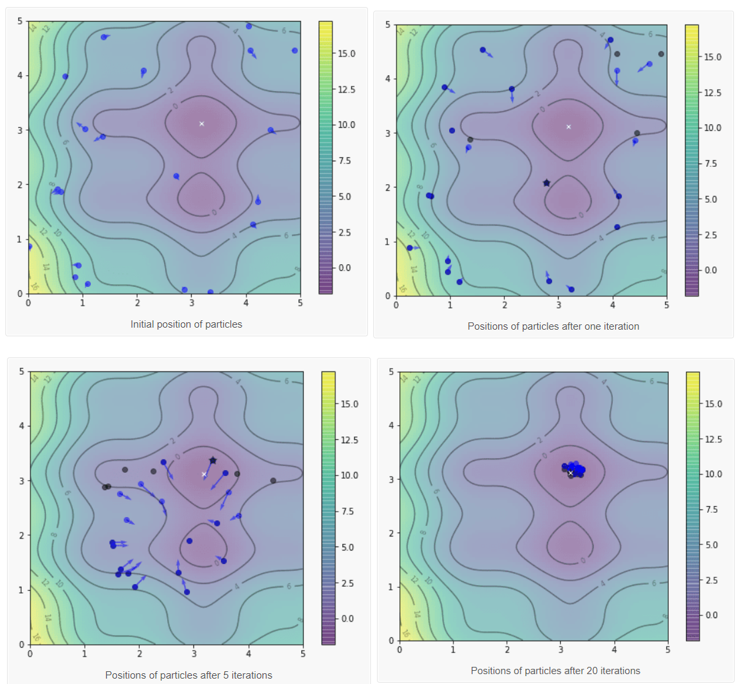
\includegraphics[width=14cm]{figures/figure-3.2.1.png}
	\caption[Visual Representation of Particle Swarm Optimization]{Visual representation of the convergence of the Particles to the Global Optimum in the Search Space in a Particle Swarm Optimization Algorithm. Source:~\cite{Tesi-3.1}}
	\label{fig:figure-3.2.1}
\end{figure}

\subsection{Components of Particle Swarm Optimization}

Particle Swarm Optimization can have better results, be faster and be cheaper compared to other methods. It is an easy problem to parallelize. Does not require the target function to be differentiable. It has few and not much complex hyperparameters.
\\[0.3cm]In short, PSO is a has a large set of advantages, it is a modern solution to perform optimization tasks. The final objective remains the same as every optimization problem, minimize (or maximize) a given function.
\\[0.3cm]The three components of PSO algorithm are: Particle, Swarm and Optimization.

\subsubsection{Particle}

The Particle Swarm Optimization is inspired by the behaviour of flocks of birds. Therefore, the term “Particle”, refers to a single individual in the Swarm.
\\[0.3cm]Every Particle is defined by its Position and their Velocity in the Search Space.
The Position in the Search Space allows for the evaluation of the values corresponding to that position, whereas the Velocity allows Particles to move stochastically in the Search Space, in seek of new better positions, and thus solutions.

\myparagraph{Initialization of Particles:}
At the start of the optimization process, the positions of the Particles are defined randomly: random values of the Search Space are assigned to the Particles.
The Velocity and direction of the Particles is also randomly generated.

\myparagraph{Evaluation of Particles:}
The Particle in the PSO is thus an agent, the position this agent has in the Search Space is a potential solution, a candidate solution.
Each Particle has Fitness values, which are evaluated by the Fitness Function, which is the function object of the optimization.
The Fitness Function evaluates a Particle's Positions, taking in input the values of the Search Space corresponding to that position.

\subsubsection{Swarm}
The Swarm is the Population of Particles of the optimization process, it represents the flock of birds.
\\[0.3cm]PSO has similarities with Genetic Algorithms, but differently from them, there are no Evolution Operators to update the individual for the next generation.
In PSO the next generation of individuals is an update of the former generation, which Position and Velocity are updated in order to improve the Fitness.

\myparagraph{Inertia, Cognitive Intuition and Social Intuition:}
After each iteration in the Search Space, the Velocity of each Particle is stochastically accelerated; consequently, also its Position will change.
\\[0.3cm]The value the Velocity is going to be updated is influenced by three factors: Inertia, Cognitive Intuition and Social Intuition. (Fig.~\ref{fig:figure-3.2.2})
\\[0.3cm]Inertia is the tendency to keep the Velocity from the previous iteration.
Cognitive Intuition is what makes the Particle accelerate toward the previous best Local Position, which is the best Position (corresponding to best Fitness) which that Particle has achieved so far.
Social Intuition is what makes the Particle accelerate toward the previous best Global Position, which is the best Position (corresponding to best Fitness) which the Particles in the Swarm have achieved so far.
\begin{figure}[t]
	\centering
	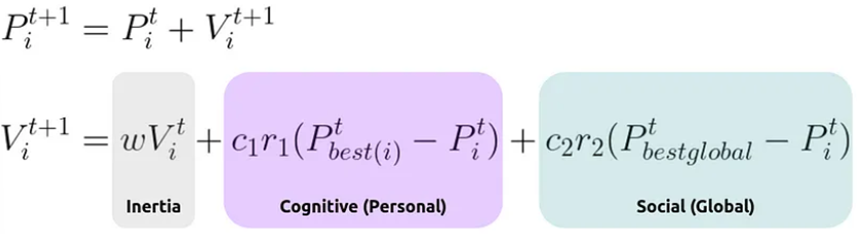
\includegraphics[width=13cm]{figures/figure-3.2.2.png}
	\caption[Alternative Update Functions for PSO]{Alternative update functions for the Velocity of the Particles in a Particle Swarm Optimization Algorithm, where the three components of the update function are represented, and additional parameters, $c_1$ and $c_2$ are introduced. Source:~\cite{Tesi-3.2}}
	\label{fig:figure-3.2.2}
\end{figure}

\subsubsection{Optimization}

The Optimization component of PSO, consists in the actual process of update of the parameters, with the correlate setting of Hyperparameters.
Inertia, Cognitive and Social coefficients have the function to control the levels of Exploitation and Exploration.
\\[0.3cm]Exploitation means to use the good solutions found so far in order to search for even better solutions in that mathematical neighbourhood. Exploration means to explore distant sections of the Search Space, in seek of new information on the Space or potentially improving solutions.

\myparagraph{Weighting of Acceleration:}
At each iteration, both the Cognitive section and the Social section of the update formula are weighted by random terms \cite{Tesi-3.2} \cite{Tesi-3.5}.
Basically, Cognitive acceleration and Social acceleration are stochastically adjusted by weights, to make the update process more random and less deterministic. The possible values that the coefficients can assume are in Fig.~\ref{fig:figure-3.2.3}.
\begin{figure}[t]
	\centering
	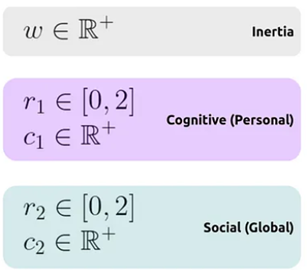
\includegraphics[width=5cm]{figures/figure-3.2.3.png}
	\caption[Values Ranges for PSO Parameters]{Ranges of values for the Parameters of a Particle Swarm Optimization Algorithm. Source:~\cite{Tesi-3.2}}
	\label{fig:figure-3.2.3}
\end{figure}

\myparagraph{Value of Inertia:}
The value of the Inertia coefficient defines the ability of the Swarm to change direction.
\\[0.3cm]Lower values of Inertia coefficient lead to better convergence; so low Inertia increases the exploitation of the best solutions.
\\[0.3cm]Higher values of Inertia coefficient increase the exploration around the best solutions.
Values too much high for Inertia, values $>1$, cause divergence of the Particles \cite{Tesi-3.2}.

\myparagraph{Value of Cognitive Coefficient:}
The value of Cognitive coefficient defines the ability of the Swarm to be influenced by the personal solutions of each Particle.
\\[0.3cm]If the Cognitive coefficient is too high, then there will be no convergence, as each individual would be too focused on its optimal solution \cite{Tesi-3.2}.

\myparagraph{Value of Social Coefficient:}
The value of Social coefficient defines the ability of the Swarm to be influenced by the best global solutions of the whole Swarm.

\myparagraph{Auto Hyperparameters:}
Inertia, Cognitive and Social coefficients are all three Hyperparameters for the optimization process of PSO.
\\[0.3cm]Searching for the optimal values of there coefficient is a complex and expensive task, as it would require another optimization process.
Moreover, the optimal value of these parameter changes during the optimization process, as the iterations go on.
\\[0.3cm]Therefore, a satisfactory solution is to update the coefficients over the iterations \cite{Tesi-3.2}.
Good reccomended update formulas, coming from empirical studies, are the equations below.
\\[0.3cm]The initial values should guarantee high exploration and more individuality, so high Inertia and Cognitive and low Social.
\\[0.3cm]Toward the end of the optimization, values should guarantee high exploitation and convergence to local optimum, so low Inertia and Cognitive and high Social.
\begin{equation}
	w = 0.4\frac{(t-N)}{N^2} + 0.4
\end{equation}
\begin{equation}
	c_1 = -3\frac{t}{N} + 3.5
\end{equation}
\begin{equation}
	c_2 = +3\frac{t}{N} + 0.5
\end{equation}

\subsection{Principles, Applications and Variants of Particle Swarm Optimization}

Principles of Swarm Intelligence, real-world applications of Particle Swarm Optimization, and PSO variants.

\subsubsection{Principles of Particle Swarm Optimization}

Particle Swarm Optimization has evolved a lot during its first experimental phase.
While it was originally meant to simulate the behaviour of a Flock of birds, the final form of the algorithm resembles more a Swarm than a Flock. For this reason, it took the name of Swarm Optimization.
\\[0.3cm]The first researcher who talked about Swarm Intelligence, Millonas \cite{SwarmIntelligence}, defined 5 principles of Swarm Intelligence.
Particle Swarm Optimization adhere to all the 5 principles.

\myparagraph{1 - Proximity Principle:}
The population should be able to perform simple space and time computations.

\myparagraph{2 - Quality Principle:}
The population should be able to respond to quality factors in the environment.
\\[0.3cm]The PSO adheres to this principle because the population, the Swarm, tend to follow the positions Local Optimum and Global Optimum, which are the environment's factors.

\myparagraph{3 - Diverse Response Principle:}
The population should ensure enough diversity in its responses.
\\[0.3cm]The PSO adheres to this principle because the responses range from the Local Optimum of the Particle and Global Optimum of the Swarm, ensuring the diversity.

\myparagraph{4 - Stability Principle:}
The population should not change its behaviour at each environmental change.
\\[0.3cm]The PSO adheres to this principle because the population only changes when the Global Optimum is updated and is therefore stable.

\myparagraph{5 - Adaptability Principle:}
The population should be able to change its behaviour when it Is worth the computational price.
\\[0.3cm]The PSO adheres to this principle because the population does change its behaviour when the Global Optimum is updated.

\subsubsection{Applications of Particle Swarm Optimization}

One of the main reasons why Particle Swarm Optimization is widely used as optimization technique, is that it is well appliable to a wide range of problems \cite{Tesi-3.4}.
The advantage of PSO is that it has a small number of Hyperparameters to set, this allow the algorithm to be easily appliable to specific applications \cite{Tesi-3.4} \cite{Tesi-3.1} \cite{Tesi-3.3} \cite{Tesi-3.5}.
\\[0.3cm]\textbf{Evolution of Neural Networks:} Particle Swarm Optimization can substitute traditional methods for the optimization of a Neural Network weights.
PSO is able to reach or outperform traditional approaches like Backpropagation.
PSO can work so well with Neural Networks, that not only can be used to optimize the networks' weights, but also their structure. PSO applies is effective for any network architecture \cite{Tesi-3.4}.
\\[0.3cm]\textbf{Human Tremor Diagnosis:} PSO has been used in combination with Neural Networks for the diagnosis of Humar Tremor conditions, for example Parkison's Disease \cite{Tesi-3.4}.
\\[0.3cm]\textbf{End Milling Manufacturing:} PSO has been used in combination with Neural Networks for End Milling manufacturing \cite{Tesi-3.4}.
\\[0.3cm]\textbf{Voltage Stability:} PSO has been used for a dynamic power and voltage control in a Japanese electric establishment \cite{Tesi-3.4}.
\\[0.3cm]\textbf{Determination of Battery State:} PSO has been used in combination with Neural Networks for estimating the state-of-charge of electrical or hybrid vehicles \cite{Tesi-3.4}.

\subsubsection{Variants of Particle Swarm Optimization}

The Particle Swarm Optimization is a popular and effective optimization technique; therefore, many variants of the approach have been developed \cite{Tesi-3.2}.
\\[0.3cm]Variants primarily focalize of adding evolutionary capabilities to PSO or improving performance with Hyperparameters.

\myparagraph{Hybrid of Genetic Algorithm and PSO (GA-PSO):}
Hybrid of Genetic Algorithm and PSO (GA-PSO) implements the mainly aspects of GA approach as the capability of breeding and crossover.

\myparagraph{Hybrid of Evolutionary Programming and PSO (EPSO):}
Hybrid of Evolutionary Programming and PSO (EPSO) implements the tournament selection in PSO, where the losing Particles changes their position.

\myparagraph{Adaptive PSO (APSO):}
Adaptive PSO (APSO) applies Fuzzy Logic to the Inertia coefficient. In addition, uses another PSO to perform the Hyperparameter Optimization for the first PSO.

\myparagraph{Multi Objective PSO (MOPSO):}
Multi Objective PSO (MOPSO) implements the concept of Pareto Dominance to determine which Particle should set the Global Optimum \cite{Tesi-3.5}.

\myparagraph{Discrete PSO (DPSO):}
Discrete PSO (DPSO) makes the performance of optimization better, for example using mixed search approach \cite{Tesi-3.5}.




\section{Analysis}

\lipsum  % Replace with your text

\section{Design}

\lipsum  % Replace with your text

\section{Implementation}

\lipsum  % Replace with your text
